% This is samplepaper.tex, a sample chapter demonstrating the
% LLNCS macro package for Springer Computer Science proceedings;
% Version 2.20 of 2017/10/04
%
\documentclass[runningheads]{llncs}
%
% !TEX root = main.tex

% Packages All the Way

\usepackage{balance,color,amsmath, alltt, xspace, epsfig, algorithm, subfigure, xcolor, multirow, psfrag,mathtools,comment, verbatim,algpseudocode,grffile}					
\usepackage{xurl}

%\usepackage[latin1]{inputenc}
\usepackage{tikz}
\usetikzlibrary{shapes,arrows}

\tikzstyle{decision} = [diamond, draw, fill=blue!20, 
text width=4.5em, text badly centered, node distance=3cm, inner sep=0pt]
\tikzstyle{block} = [rectangle, draw, fill=blue!20, 
text width=5em, text centered, rounded corners]
\tikzstyle{line} = [draw, -latex']

\tikzstyle{cloud} = [draw, ellipse,fill=red!20, node distance=3cm,
minimum height=2em]

 \usepackage{graphicx} 
\usepackage{caption}
\captionsetup[figure]{font=small}
%\usepackage[hyphens]{url}
\usepackage{hyperref}
\hypersetup{breaklinks=true}


% Variable Part
\newcommand{\algoname}{DALock}					%Give a name to the algorithm/theorem


\newcommand{\authnote}[3]{\textcolor{#2}{{\sf (#1's Note: {\sl{#3}})}}}
\newcommand{\wuwei}{\authnote{Wuwei}{green}}
\newcommand{\jeremiah}{\authnote{Jeremiah}{blue}}
\newcommand{\ignore}[1]{}

% Fixed/Constant Part:
%\newtheorem{theorem}{Theorem}
%\newtheorem{definition}{Definition}
\newcommand{\mypara}[1]{\noindent\textbf{#1} \xspace}		% Bold paragraph title
\newcommand{\says}[2]{{\color{blue}{#1 says: }{#2}}\xspace}					% Says 
\DeclarePairedDelimiter{\ceil}{\lceil}{\rceil}								%\ceil	

%---------- Macros for Table (Below)-------------
\newcommand{\PasswordOfU}[1]{pw_{#1}}
\newcommand{\PwOfU}[1]{pw_{#1}}
\newcommand{\PsiOfU}{\Psi_u}
\newcommand{\KOfU}{K_u}
\newcommand{\PwProbEstimator}{\mathsf{Est}}
\newcommand{\AllUser}{\mathcal{U}}
\newcommand{\RankRPassword}[1]{pw_{#1}}
\newcommand{\user}{u}
\newcommand{\Lap}{\mathsf{Lap}\xspace}								% Laplace Noise
\newcommand{\epsLap}[2]{\ensuremath{\mathsf{LAP(\frac{#2}{#1})}}\xspace} %Laplace Noise with #1 privacy budget (\epsilon) and #2 sensitivity
\newcommand{\Adversary}{\ensuremath{\mathcal{A}}}							% Lazy \mathcal{A}
\newcommand{\lazyref}[2]{\textbf{#1}~\ref{#2}}
\newcommand{\ZX}{\ZXCVBN} 			%Lazy fancy ZXCVBN
\newcommand{\loginActivity}[3]{\mathsf{L_{#1}(#2,#3)}}
\newcommand{\ZXCVBN}{\mathsf{ZXCVBN}}
\newcommand{\PCFG}{\mathsf{PCFG}}
\newcommand{\Min}{\mathsf{Min}}
\newcommand{\HashCat}{\mathsf{HashCat}}
\newcommand{\NeuralNet}{\mathsf{NeuralNet}}
\newcommand{\Markov}{\mathsf{Markov}}
\newcommand{\Estimator}{\mathsf{Estimator}}
\newcommand{\EstF}[1]{\textsf{Estimate}(#1)}
\newcommand{\EstimateF}[2]{\textsf{Estimate}(#1,#2)}			%Estimate Frequency of p 
\newcommand{\EstP}[1]{\textsf{p}(#1)}
\newcommand{\EstimateP}[2]{\textsf{p}(#1,#2)}			%Estimate popularity of p 
\newcommand{\MM}{\ensuremath{\mathcal{M}}}							% Lazy \mathcal{A}
\newcommand{\FMPPF}{\ensuremath{\mathsf{FMPPF}}}							% Lazy \mathsf{FMPPF}
\newcommand{\DAB}{\ensuremath{\mathsf{DAB}}}	
\newcommand{\PK}{\ensuremath{\mathsf{PK}}}							% Lazy Password Knapsack
\newcommand{\SampledData}[1]{\mathcal{D}_{{#1}}}
\renewcommand{\Pr}[1]{\ensuremath{\mathsf{Pr} \left[#1\right] }\xspace}			% Fancy Pr
\newcommand{\KPsiDALock}[2]{\ensuremath{(#1, #2)\text{-}\mathsf{DALock}}\xspace}		
\newcommand{\hitCountThreshold}{\Psi}
\newcommand{\hitCountThresholdOfU}[1]{\hitCountThreshold_{#1}}	
\newcommand{\DP}[2]{\textsf{DP}(#1,#2)}
\newcommand{\strikeThreshold}{K}	
\newcommand{\strikeThresholdOfU}[1]{\strikeThreshold_{#1}}
\newcommand{\DALock}{\mathsf{DALock}\xspace}	
\newcommand{\AllPassword}{\mathcal{P}}
\newcommand{\CountSketch}{\mathsf{CS}}
\newcommand{\CountSketchCounter}{\mathsf{CS.T}}
\newcommand{\CountSketchArray}{\mathsf{CS.ARRAY}}
\newcommand{\EstProbOfPw}[2]{\ensuremath{\Estimator_{\mathsf{#2}}}\left(#1\right)}
\newcommand{\TrueP}[1]{\ensuremath{\mathsf{P}\left(#1\right)}}
\newcommand{\TrueF}[1]{\ensuremath{\mathsf{F}\left(#1\right)}}
\newcommand{\TrueFInD}[2]{\ensuremath{\mathsf{F}\left(#1, #2\right)}}
\newcommand{\CSWidth}{w}
\newcommand{\CSDepth}{d}
\newcommand{\TotalFreq}[1]{\ensuremath{\mathsf{TotalFreq}(#1)}}
\newcommand{\Add}[2]{\ensuremath{\mathsf{Add}(#1,#2)}}
\newcommand{\Initialize}[2]{\ensuremath{\mathsf{Initialize}(#1,#2)}}
\newcommand{\HashFunRowD}{\ensuremath{\mathsf{h}_d}}
\newcommand{\HashFunSign}{\ensuremath{\mathsf{h}_{\pm}}}
\newcommand{\hitCountThresholdofUAtT}[2]{\hitCountThresholdOfU{#1}^{#2}}
\newcommand{\strikeThresholdofUAtT}[2]{\strikeThresholdOfU{#1}^{#2}}
%---------- Macros for Table (Above)-------------


\newtheorem{definition}{Definition}
\newtheorem{thm}{Theorem}[section]
\newcommand{\NP}{\mathsf{NP}\xspace}

\newcommand{\FPTAS}{\mathsf{FPTAS}\xspace}
\newcommand{\PTAS}{\mathsf{PTAS}\xspace}
\renewcommand{\P}{\mathsf{P}\xspace}	
\newcommand{\SAT}{\mathsf{SAT}\xspace}	
\newcommand{\TIME}{\mathsf{TIME}\xspace}
\newcommand{\NPC}{\mathsf{NPC}\xspace}	
\newcommand{\myexp}[1]{\ensuremath{e^{#1}}\xspace}						% exp


%---------- Macros for General Setting-------------
\algrenewcommand\algorithmicindent{1.0em}%
\usepackage{tikz}
\usetikzlibrary{matrix,calc,shapes}
\tikzset{
  treenode/.style = {shape=rectangle, rounded corners,
                     draw, anchor=center,
                     text width=5em, align=center,
                     top color=white, bottom color=blue!20,
                     inner sep=1ex},
  decision/.style = {treenode, diamond, inner sep=0pt},
  root/.style     = {treenode, font=\Large, bottom color=red!30},
  env/.style      = {treenode, font=\ttfamily\normalsize},
  finish/.style   = {root, bottom color=green!40},
  dummy/.style    = {circle,draw}
}
\newcommand{\yes}{edge node [above] {yes}}
\newcommand{\no}{edge  node [left]  {no}}




\usepackage[strings]{underscore}
\usepackage{graphicx}
% Used for displaying a sample figure. If possible, figure files should
% be included in EPS format.
%
% If you use the hyperref package, please uncomment the following line
% to display URLs in blue roman font according to Springer's eBook style:
% \renewcommand\UrlFont{\color{blue}\rmfamily}

\begin{document}
%
\title{$\DALock$: Password \underline{D}istribution-\underline{A}ware Throttling}
%
%\titlerunning{Abbreviated paper title}
% If the paper title is too long for the running head, you can set
% an abbreviated paper title here
%
\author{Anonymous submission}
%
%\authorrunning{F. Author et al.}
% First names are abbreviated in the running head.
% If there are more than two authors, 'et al.' is used.
%
%\institute{Princeton University, Princeton NJ 08544, USA \and
%Springer Heidelberg, Tiergartenstr. 17, 69121 Heidelberg, Germany
%\email{lncs@springer.com}\\
%\url{http://www.springer.com/gp/computer-science/lncs} \and
%ABC Institute, Rupert-Karls-University Heidelberg, Heidelberg, Germany\\
%\email{\{abc,lncs\}@uni-heidelberg.de}}
%
\maketitle              % typeset the header of the contribution
%
\begin{abstract}
\input{abstract}

\keywords{First keyword  \and Second keyword \and Another keyword.}
\end{abstract}
\input{TBD}
%
%
%
\input{paperBody} 

%
%
% \bibliography{mybibliography}
%

\bibliographystyle{splncs04}
\bibliography{../cryptobib/abbrev0,../cryptobib/crypto,../otherReference/otherRef}
% !TEX root = main.tex

\appendix




\subsection{$\DALock$ Authentication Algorithm}
We supplement the pseudo code of $\DALock$ in this section to help readers understand how to implement $\DALock$. The authentication process takes four arguments: username $u$, input password $pw$ (which may or may not be the same as $u$’s password $pw_u$), salt $s_u$, and password popularity estimator $\sigma$. Before verifying the correctness of the entered password, $\DALock$ first checks if $u$'s account has already been locked or not based on $\hitCountThreshold_{u}$ and $\strikeThreshold{u}$. If the account is not locked, $\DALock$ proceeds and verifies the correctness of the entered password. If the password is valid, i.e., pw = $pw_u$, $\DALock$ resets strike threshold $\strikeThresholdOfU{u}$ and grants the access. If the entered password is wrong, then in addition to denying access to the service, the server also increases $\hitCountThresholdOfU{u}$ and $\strikeThreshold$ by $\EstP_{\sigma}{pw}$ and 1, respectively.


\begin{algorithm}[!htb]
	\caption{\textbf{$\DALock$}: Novel Password Distribution-Aware Throttling Mechanism }\label{algorithm:DALock}
	\begin{algorithmic}[1]
		\Function{login}{$u$, $pw_u$, $\sigma$,$s_u$} 
		\If {$\hitCountThresholdOfU{u} \geq \hitCountThreshold$ or  $\strikeThresholdOfU{u} \geq \strikeThreshold$ }
		\State Reject Login(Locked)
		\EndIf
		\If{$hash(pw,s_u)$ == $hash(pw_u,s_u)$}
		\State Reset $\strikeThresholdOfU{u}$ to 0
		\State Grant Access
		\Else
		\State $\hitCountThresholdOfU{u} \leftarrow \hitCountThresholdOfU{u} + \EstimateP{pw}{\sigma}$
		\State $\strikeThresholdOfU{u} \leftarrow \strikeThresholdOfU{u}$ + 1
		\State Deny Access
		\EndIf
		\EndFunction
	\end{algorithmic}
\end{algorithm} 
\vspace{-0.5cm}
\subsection{Password Knapsack is $\NP$ hard}\label{appendix:pkhardness}

In this section, we supplement the details on proving $\PK$ is $\NP$ hard by showing a reduction from a well-known $\NP$hard problem subset-sum to it. We begin this by first formally define the subset sum problem and then prove password knapsack is $\NP$ hard by showing the reduction from subset sum to it.

\begin{definition}[Subset Sum]
	Given partition instance $x_1,\ldots,x_{n} \in (0,2^m]$ and target sum value $T$. The  goal is to find $S \subseteq [n]$ s.t. $\sum_{i\in S} x_i = T$.
\end{definition}

\begin{thm}[Hardness of Password Knapsack]\label{appendix:ProofOfPasswordKnapsack}
	Find optimal solutions for password knapsack is $\NP$-hard.
\end{thm}

\mypara{Proof:}
\textbf{Reduction}: One can create the following password knapsack instance 
\begin{itemize}
	\item Set $\gamma = \sum_{i=1}^n x_i$,
	\item Set $\psi = T/(2\gamma )< \frac{1}{2}$,
	\item Set $CS(p_i)= f(p_{i}) = x_i/(2\gamma)$ for $i=1,\ldots, n$
	\item Set $f(p_{last}) = 1-\sum_{i =1}^{n} p_i = 1/2 > \psi$. 
\end{itemize}
If $S$ exists for partition instance, then the attacker can use $S$ for password knapsack to crack $p_{last}+T/(2\gamma)$ passwords. On the other hand, let $S$ be the optimal password knapsack solution such that $\sum_{i \in S} CS(p_i) \leq \psi$, then the attacker cracks at most $p_{last}+\sum_{i \in S} f(p_i) \leq 1/2 + \psi$ passwords. If equality holds, then $\sum_{i \in S} f(p_i) = \psi$ which implies $\sum_{i \in S} x_i = T$ by definition of $\psi$.





\subsection{Solving $\PK$ with Heuristic}\label{appendix:solvePK}
In this section, we discuss two heuristic approaches, $\DAB$ and $\FMPPF$, described in \lazyref{Section}{section:ExperimentDesign-subsection:SimulateAttacker}.  

The $\DAB$ approach takes three inputs: a sorted password dictionary $\mathcal{P}_{\tilde{\Pi}} = \{\tilde{pw}_1, \ldots, \tilde{pw}_{n} \}$, hit count budget $\hitCountThreshold$ and strike count budget $\strikeThreshold$. $\mathcal{P}_{\tilde{\Pi}}$ is sorted based on the ratio of actual popularity and estimated popularity, i.e., $\frac{\EstP{pw}}{\TrueP{pw}}$: $\mathcal{P}_{\tilde{\Pi}} = \{pw_{\tilde{\Pi}(1)}, \ldots, pw_{\tilde{\Pi}(n)} \}$. The algorithm keeps placing passwords into the knapsack S based on the sorted order until it cannot further add some password $pw$, i.e., $\EstP{S \cup pw} \ge \hitCountThreshold$. At this point, $\DAB$ compares $\TrueP{pw}$ with $\TrueP{S}$ and sets S to be the one with the higher value. The above process is repeated until the whole dictionary is scanned. In the end, the algorithm returns $K$ passwords based on their actual probabilities.

Primary incentives of using $\DAB$ are 1) to take advantage of underestimated passwords and 2) to avoid (severely) overestimated ones. However, there are several drawbacks of $\DAB$. Firstly, the progress can be slow because priorities are given to significantly underestimated passwords, i.e., rare passwords. Intuitively, the ratio $\frac{\TrueP{pw}}{\EstP{pw}}$ of popular password $pw$, i.e., $\TrueP{pw}$ is large, is likely to be close to 1; therefore, attempts with popular ones are likely to be delayed. Secondly, unlike the vanilla version of Knapsack, $\DAB$ may not yield a 2-approximation due to the additional constraint on the number of passwords. Third, the computation cost of $\DAB$ is high because the algorithm has to go through the whole dictionary (for each run). Consider $\Adversary$ usually attack multiple accounts simultaneously, $\DAB$ may not be the heuristic to be used.
%is slightly higher for running $\DAB$ though both algorithms terminate reasonably quickly. %Thirdly, computation cost can still be a concern for large scale attacks. 



%\begin{algorithm}[!htb]
%	\caption{\textbf{$\DAB$ Attack }}\label{algorithm:Dantizig}
%	\textbf{Return:}  An array of password sorted in the order of guessing
%	\begin{algorithmic}[1]
%		\Function{$\DAB$ Attack}{$\mathcal{P}_{\tilde{\Pi}}, \Psi, M(T)$}
%		\State $S$= []
%		\While{$S$ changes}
%		\For{ $pw \in \mathcal{P}_{\tilde{\Pi}}$  }
%		\If{$\EstP{pw}$ $> \Psi$ }
%		\State \textbf{continue}
%		\EndIf
%		\If{$\EstP{S\cup pw}$ $< \Psi$ and $|S| \le$ $M(T)$  }
%		\State $S \leftarrow S \cup pw$ 
%		\ElsIf{$\TrueP{pw} > \TrueP{S}$ }
%		\State $S \leftarrow$ \{p\}
%		\EndIf
%		\EndFor
%		\EndWhile
%		\State \Return Top $M(T)$ passwords from $S$ based on actual popularity.
%		\EndFunction
%	\end{algorithmic}
%\end{algorithm}  

%and its pseudo code is available in \textbf{Algorithm}~\ref{algorithm:FMPPF}. 
A faster alternative to $\DAB$ is $\FMPPF$.  It takes three input parameters: password dictionary $\mathcal{P} = \{pw_1, \ldots, pw_{n} \}$, hit count budget $\hitCountThreshold$, and strike budget $\strikeThreshold$. $\FMPPF$ selects passwords greedily as well but using different criteria. $\mathcal{P}$ is a password dictionary sorted based on the actual popularity only. In addition, to save computational cost, $\FMPPF$ terminates once it finds $K$ passwords suitable for attacks and stops further exploring the dictionary.

In short-time attack scenarios, $\FMPPF$ offers a better chance of success than $\DAB$ by attempting popular ones first. For long-term attacks, $\FMPPF$ should still be able to achieve almost optimal results given an abundant choice of passwords.  In fact, based on the empirical results (in \textbf{section}~\ref{section:ExperimentResult-security}), the performance of $\FMPPF$ is very close to theoretical upper bounds ($\Psi + \TrueP{pw_1}$) . %Last but not least, $\FMPPF$ is computational efficient comparing to $\DAB$.


%\begin{algorithm}[!htb]
%	\caption{\textbf{$\FMPPF$ Approach}}\label{algorithm:FMPPF}
%	\textbf{Return:} An array of password sorted in the order of guessing
%	\begin{algorithmic}[1]
%		\Function{\FMPPF}{$\mathcal{P}, \Psi, M(T)$}
%		\State $S$= []
%		\For{ $pw \in \mathcal{P}$  }
%		\If{$\EstP{S \cup p}$ $< \Psi$ and $|S| < M(T)$  }
%		\State $S \leftarrow S \cup pw$ 
%		\EndIf
%		\EndFor
%		\State \Return S
%		\EndFunction
%	\end{algorithmic}
%\end{algorithm} 


\subsection{Details on Simulating Users' Mistakes}\label{appendix:simulateMistakes}
In this section, we elaborate on the missing details for simulating users' mistakes. To help readers visualize the process, we plot a flowchart in \textbf{figure}~\ref{figure:flowChartTypo}. The starting point is to simulate the recall error. Following existing works \cite{CCS:CWPCR17,SP:CAAJR16}, we set the probability of making a recall error to be 2.4\%. When making a recall error, we assume that each user will choose one of their five ``passwords from other services" uniformly, i.e., w.p. 20\%. After this step, we further simulate typos (on the password intended to enter) w.p. approx. 5\%. Condition on making typos, we simulate this step by choosing a typo type with their conditional probability summarized in \textbf{Table}~\ref{Table:TypoTypes}(e.g., insert an extra letter w.p. 12\%.). Notice that a user can make both mistakes. e.g., recall the wrong password $pw$' and typo $pw$'.

\begin{figure}
		% !TEX root = ../../main.tex
\resizebox{\linewidth}{5cm}{
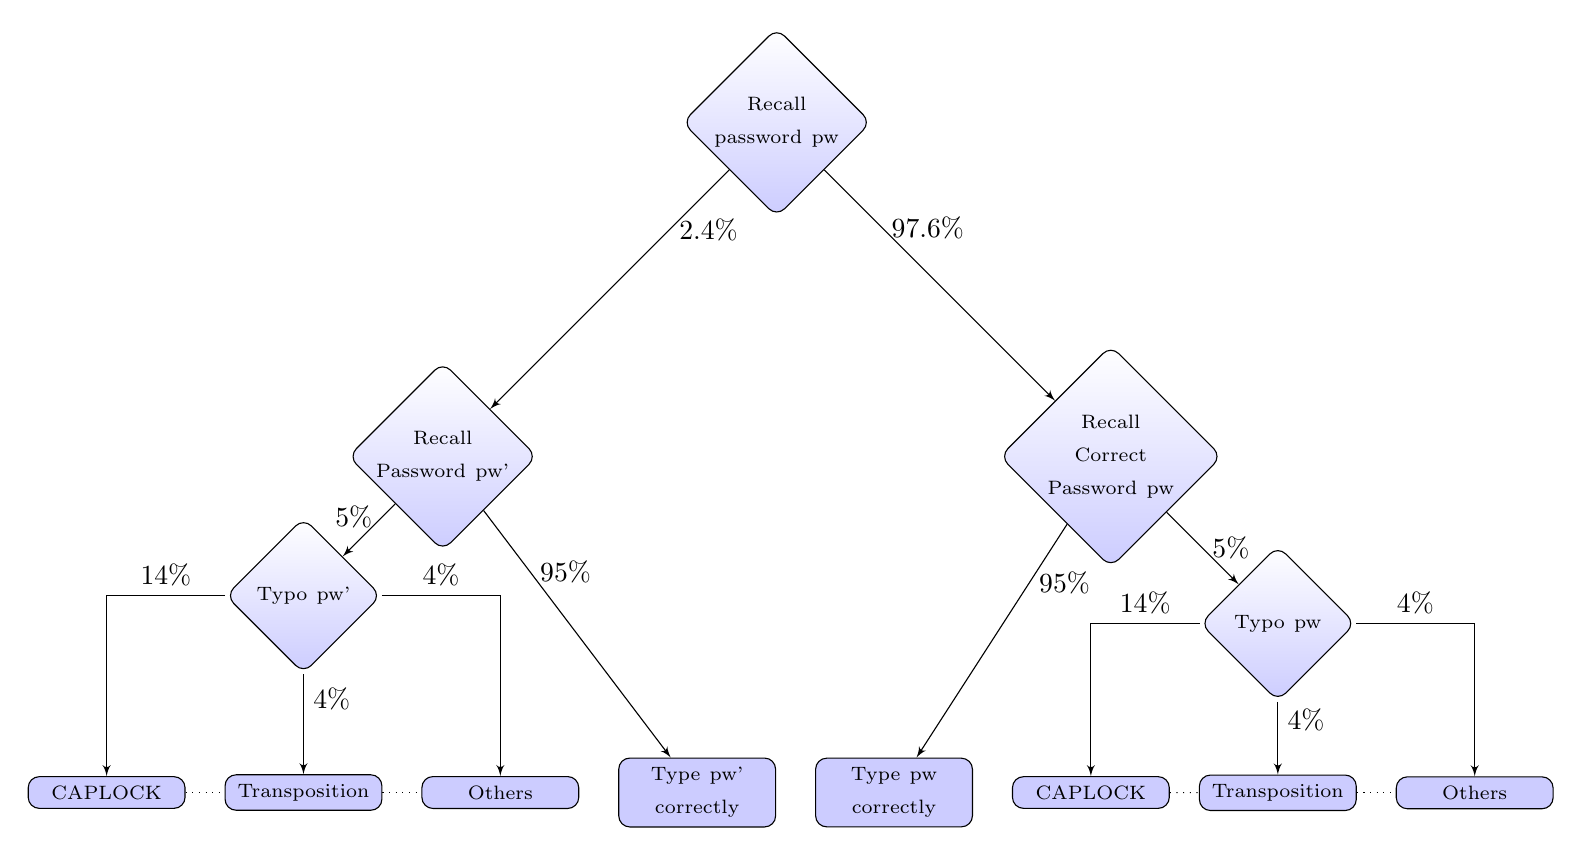
\begin{tikzpicture}
	% Place nodes
	\node [decision] (choosepwd) {\scriptsize{Recall password pw}};    
	% Level 2
	
	\node [decision,  below left of=choosepwd,node distance=6cm] (wrongPwd) {\scriptsize{Recall Password pw'}}; \path [line] (choosepwd) -- node [near start,right] {2.4\%} (wrongPwd);
	% Level 3
	\node [decision, below left of=wrongPwd,node distance=2.5cm](wrongPwdTypo){\scriptsize{Typo pw'}}; \path [line] (wrongPwd) -- node [near start, left] {5\%}(wrongPwdTypo);
	% Level 4
	\node [block,below of=wrongPwdTypo,node distance=2.5cm](wrongPwdTypoTrans){\scriptsize{Transposition}}; \path [line] (wrongPwdTypo) -- node [near start, right] {4\%}(wrongPwdTypoTrans);
		\node [block, left of=wrongPwdTypoTrans,node distance=2.5cm](wrongPwdTypoCap){\scriptsize{CAPLOCK}}; \path [line] (wrongPwdTypo) -| node [near start,above] {14\%}(wrongPwdTypoCap);
	\node [block, right of=wrongPwdTypoTrans,node distance=2.5cm](wrongPwdTypoOther){\scriptsize{Others}}; \path [line] (wrongPwdTypo) -| node [near start,above] {4\%}(wrongPwdTypoOther);
	\node [block, right of=wrongPwdTypoOther, node distance = 2.5cm](wrongPwdCorrect){\scriptsize{Type pw' correctly}};\path [line] (wrongPwd) -- node [near start,right] {95\%} (wrongPwdCorrect);
	
	\node [decision,  below right of=choosepwd,node distance=6cm] (rightPwd) {\scriptsize{Recall Correct Password pw}};             \path [line] (choosepwd) -- node [near start,right] {97.6\%}(rightPwd);
	% Level 3
	\node [decision, below right of=rightPwd,node distance=3cm](rightPwdTypo){\scriptsize{Typo pw}}; \path [line] (rightPwd) -- node [midway,right] {5\%}(rightPwdTypo);
	% Level 4
		\node [block, right of=wrongPwdCorrect, node distance = 2.5cm](rightPwdCorrect){\scriptsize{Type pw correctly}};\path [line] (rightPwd) -- node [near start,right] {95\%} (rightPwdCorrect);
			\node [block, below of=rightPwdTypo,node distance=2.15cm](rightPwdTypoTrans){\scriptsize{Transposition}}; \path [line] (rightPwdTypo) -- node [near start,right] {4\%}(rightPwdTypoTrans);
	\node [block, right of=rightPwdCorrect,node distance=2.5cm](rightPwdTypoCap){\scriptsize{CAPLOCK}}; \path [line] (rightPwdTypo) -| node [near start,above] {14\%}(rightPwdTypoCap);

	\node [block, right of=rightPwdTypoTrans,node distance=2.5cm](rightPwdTypoOther){\scriptsize{Others}}; \path [line] (rightPwdTypo) -| node [near start,above] {4\%}(rightPwdTypoOther);
	 \draw [dotted] (wrongPwdTypoCap) -- (wrongPwdTypoTrans);
	 	\draw [dotted] (wrongPwdTypoTrans) -- (wrongPwdTypoOther);
	 		 \draw [dotted] (rightPwdTypoCap) -- (rightPwdTypoTrans);
	 	\draw [dotted] (rightPwdTypoTrans) -- (rightPwdTypoOther);
	%\node [block, below of=identify] (evaluate) {evaluate candidate models};
	%\node [block, left of=evaluate, node distance=2.5cm] (update) {update model};
	% \node [decision, below of=evaluate] (decide) {is best candidate better?};
	%\node [block, below of=decide, node distance=2.5cm] (stop) {stop};
	% Draw edges
	
	
	%\path [line] (identify) -- (evaluate);
	%\path [line] (evaluate) -- (decide);
	% \path [line] (decide) -| node [near start] {yes} (update);
	%\path [line] (update) |- (identify);
	% \path [line] (decide) -- node {no}(stop);
	
\end{tikzpicture}
}
	\caption{Flow Chart for Simulating Users' mistake}\label{figure:flowChartTypo}
\end{figure}


\begin{table}[h]
	\begin{tabular}{|c|c|}
		\hline
		Typo Types           & Chance of Mistake(Rounded \%) \\ \hline
		CapLock On           & 14                            \\ \hline
		Shift First Char     & 4                             \\ \hline
		One Extra Insertion  & 12                            \\ \hline
		One Extra Deletion   & 12                            \\ \hline
		One Char Replacement & 31                            \\ \hline
		Transposition        & 4                             \\ \hline
		Two Deletions         & 3                             \\ \hline
		Two Insertions        & 3                             \\ \hline
		Two Replacements      & 10                            \\ \hline
		Others               & 8                             \\ \hline
	\end{tabular}
	\caption{Typo Distributions\cite{CCS:CWPCR17}}
	\label{Table:TypoTypes}
	\vspace{-0.5cm}
\end{table}	


\subsection{More Experimental Results}\label{appendix:experimentalResults}
In this section, we provide more detailed experimental results for readers to understand the underlying details of $\DALock$. We elaborate on each frequency oracle's security and usability performance with wider $\hitCountThreshold$ range: $\{2^{-8}, 2^{-9},2^{-10},2^{-11}, 2^{-12}\}$. For count sketch implementation, we show extra results on applying subsampling and differential privacy with the following testing parameters:
\begin{itemize}
	\item Subsampling rate: 1\%, 5\%, 10\%, 100\%(all)
	\item Differential privacy budget: 0.1, 0.5, 1.0, $\infty$
\end{itemize}

In addition, we ran the experiments on two extra datasets: LinkedIn and Yahoo!. Since the Yahoo! dataset~\cite{SP:Bonneau12,NDSS:BloDatBon16} only contains frequencies without actual passwords. i.e., instead of recording the pair $(pw,  \TrueFInD{pw}{\SampledData{\AllUser} })$ the dataset simply records $\TrueFInD{pw}{\SampledData{\AllUser} }$ . We generate a complete password dataset by designating a unique string for each password. Thus, we avoid using password models like $\ZX$ to analyze $\DALock$ with the Yahoo! dataset since frequency estimation requires access to the original passwords. However, we are still able to evaluate $\DALock$ with the Yahoo! dataset using the count sketch frequency oracle. 

We begin by discussing the pros and cons of each frequency oracle based on our results. And then provide our insights on how to deploy $\DALock$ with it. Finally, we make our overall recommendation by comparing the performance of them.


\mypara{PCFG/NeuralNet/Markov/HashCat/Min}\footnote{Experiments results of PCFG, Markov, and Min are available in the full version of the paper. PCFG, Markov, and Min share similar security/usability trends with the Neural Network model; thus we choose to omit these three models in this paper due to space limitation.  }  \lazyref{Figure}{fig:securityneuralnet} to \lazyref{Figure}{fig:usabilityzxcvbn} demonstrate the security and usability performance of these five implementations across all datasets. As mentioned previously, those models use ``guessing number" to indicate the strength of passwords. Based on our observation, they have their best security/usability advantages (compared to the 3-stikes mechanism) when high $\hitCountThreshold$ is used and ban-list size $|B|$ is small. We notice that adopting larger $\hitCountThreshold$ hardly impacts security performance despite the fact that usability can be benefited. In fact, We only observe noticeable security impact on the Hashcat model based on brazzers, clixsense, and rockyou datasets(\lazyref{Figure}{fig:securityhashcat}).

All those frequency oracles can be used to implement $\DALock$ to achieve better security than the 3-strikes mechanism; however, they gradually lose the security advantages as the ban-list size increases, e.g., banning 100 passwords results in worse security compared to the 3-strikes mechanism on all datasets. For usability, all five implementations can be configured to have lower lockout rates than the 3-strikes mechanism. e.g., using $\hitCountThreshold \ge 2^{-9}$ results in strictly better usability than the 3-strikes mechanism across all datasets for all models. 

Based on our observation, deploying $\DALock$ with those five frequency oracles is not recommended if the server can accurately identify and ban approx. 100 popular passwords. In addition, larger $\hitCountThreshold$ is recommended, e.g., using $\hitCountThreshold = 2^{-9}$ to achieve strictly better security/usability performance compared to the 3-strikes mechanism.


\mypara{ZXCVBN} We present our security and usability findings on $\ZXCVBN$ in \lazyref{Figure}{fig:securityzxcvbn} and \lazyref{Figure}{fig:usabilityzxcvbn}. To achieve the optimal security/usability trade-off, we recommend deploying $\ZXCVBN$ with $\hitCountThreshold =2^{-9}$ combined with a large ban-list. Unlike the previously mentioned five estimators, $\hitCountThreshold$ impacts both security and usability performance sensitively. On the positive side, one can also sharpen \textit{both} the security and usability by adopting larger ban-list, e.g., B = 1000.

$\DALock$ can be easily implemented by $\ZXCVBN$ to achieve strictly better security \textit{and} usability\footnote{In \lazyref{Figure}{fig:usabilityzxcvbn}, usabiliity is close to 0 when the ban-list size is $10^5$. Notice that $\EstP{pw}$ is normalized by the top $10^5$ passwords in this case.} compared to the 3-strikes mechanism. \lazyref{Figure}{fig:securityzxcvbn} shows that adopting any $\hitCountThreshold \le 2^{-8}$ results in security advantage (compared to the 3-strikes mechanism) across all datasets even with a large ban-list; however, we do observe that $\ZXCVBN$ overestimate many rare passwords. Thus, it's crucial to adopt $\hitCountThreshold \ge 2^{-9}$ for usability practice based on $\lazyref{Figure}{fig:usabilityzxcvbn}$. Combining the security and usability results, we conclude that using $\hitCountThreshold = 2^{-9}$ yields the optimal security/usability trade-off. i.e. ZXCVBN(K:10,$\hitCountThreshold$:$2^{-9}$) is more secure than the 3-strikes mechanism and has approx. 0\% lockout rate.

In conclusion, deploying $\DALock$ with $\ZXCVBN$ is recommended when it is hard to obtain accurate password distribution description. Based on the empirical results, setting $\hitCountThreshold = 2^{-9}$ \textit{and} banning popular passwords yields the best security/usability trade-off.


\mypara{Differentially Private Count Sketch} In this section, we focus discussion on the impact of the following three parameters: hit-count $\hitCountThreshold$(\lazyref{Figure}{fig:securitypsicompare} and \ref{fig:usabilitypsicompare}), sampling rate r(\lazyref{Figure}{fig:securitysamplecompare} and \ref{fig:usabilitysamplecompare}), and privacy budget $\epsilon$(\lazyref{Figure}{fig:securitydpcompare} and \ref{fig:usabilitydpcompare}).

Tunning $\hitCountThreshold$ for optimal security/usability trade-off on a differentially private Count Sketch is a less challenging task compared to other frequency oracles. \lazyref{Figure}{fig:securitypsicompare} and \ref{fig:usabilitypsicompare} show that 0.1-CS-all can achieve strictly better security and usability than the 3-strikes mechanism for $\hitCountThreshold$ $\in$ [$2^{-8},2^{-10}$] on all datasets and with all ban-list sizes. In addition, we observe that 0.1-CS-all reaches approx. 0\% lockout rate if 100 or more passwords are banned when $\hitCountThreshold$ $\in$ [$2^{-8},2^{-10}$]. 

To investigate how many users one needs to accurately build a differentially private count sketch, we train count sketches with subsampled datasets - $\SampledData{\AllUser_{1\%}}$, $\SampledData{\AllUser_{5\%}}$, and $\SampledData{\AllUser_{10\%}}$ - in addition to $\SampledData{\AllUser}$ . \lazyref{Figure}{fig:securitysamplecompare} and \ref{fig:usabilitysamplecompare} show that lower sampling rates can hurt security as $\Adversary$ can take advantage of underestimated passwords. We also observe that  0.1-CS-10\%/0.1-CS-5\%/0.1-CS-1\% can be just as accurate as 0.1-CS-all when we have more than 2/6/32 millions users in the $\SampledData{\AllUser}$(see clixsense/csdn/RockYou). This result empirically shows organizations need approx. 0.2-0.3 million users to train an \textit{accurate} differentially private Count Sketch. 

To study how privacy noise can perturb security/usability performance of well-tuned differentially privacy Count-Sketch (e.g., with throttling parameters k = 10 and $\hitCountThreshold$ = $2^{-10}$) in bad scenarios, we experiment training Count Sketch on small datasets (e.g., $\SampledData{\AllUser_{1\%}}$) with practically small privacy budgets. \lazyref{Figure}{fig:securitydpcompare} and \ref{fig:usabilitydpcompare} demonstrate the security/usability performance of three different differentially Count-Sketches: 0.1-CS-1\%, 0.5-CS-1\%, and 1.0-CS-1\%.  \lazyref{Figure}{fig:securitydpcompare} and \ref{fig:usabilitydpcompare} also include the following baselines for comparisons: $\infty$-CS-1\% (noise-free)), 3-strikes, and 10-strikes. Based on the results, we observe that even 0.1-differential privacy had minimal impact on both security and usability performance of Count Sketches. 

In brief, the empirical results show that differentially private Count Sketch can be easily trained with low privacy budget cost, e.g., $\epsilon = 0.1$ and with as few as 0.2-0.3 million users. It's also the easiest frequency oracle to tune for security/usability performance. We recommend large entities to deploy $\DALock$ with differentially private Count Sketch once the above criteria can be met.

\mypara{Deploying $\DALock$} we found two feasible solutions to instantiate $\KPsiDALock{10}{\hitCountThreshold}$ based on experimental results - differentially private count sketches and $\ZXCVBN$ password strength meter. We recommend deploying $\DALock$ with a 0.1-differentially private count sketch with $\hitCountThreshold$ $\in$ [$2^{-8},2^{-10}$] when the authentication server can collect at least 0.3 million passwords. Otherwise we recommend using $\ZXCVBN(K:10,\hitCountThreshold:2^{-9})$ to instantiate $\DALock$. Banning popular passwords is recommended for both apporaches to achieve better security/usability results. 



\begin{figure*}
	\includegraphics[width=\linewidth, height = 8cm]{Figures/Experiments/B0.png}
	\vspace{-0.2in}
	\caption[Usability/Security Trade-off]{Usability/Security Trade-off(Banlist Size = 0)}
	\label{fig:secuseB0}
	\includegraphics[width=\linewidth, height = 8cm]{Figures/Experiments/B10.png}
	\vspace{-0.2in}
	\caption[Usability/Security Trade-off]{Usability/Security Trade-off(Banlist Size = 10)}
	\label{fig:secuseB10}
	\includegraphics[width=\linewidth, height = 8cm]{Figures/Experiments/B100.png}
	\vspace{-0.2in}
	\caption[Usability/Security Trade-off]{Usability/Security Trade-off(Banlist Size = 100)}
	\label{fig:secuseB100}
\end{figure*}

	\begin{figure*}
		\includegraphics[width=\linewidth, height = 8cm]{Figures/Experiments/B1000.png}
		\vspace{-0.2in}
		\caption[Usability/Security Trade-off]{Usability/Security Trade-off(Banlist Size = 1000)}
		\label{fig:secuseB1000}
		\includegraphics[width=\linewidth, height = 8cm]{Figures/Experiments/Attacker/SecurityBigPictureFull}
		\vspace{-0.2in}
		\caption{Security Measurement of $\DALock$ (All Datasets)}
		\label{fig:securitydpcomparefull}	
		\includegraphics[width=\linewidth, height = 8cm]{Figures/Experiments/Utility/UsabilityBigPictureFull}
		\vspace{-0.2in}
		\caption{Usability Measurement of $\DALock$(All Datasets)}
		\label{fig:usabilitydpcomparefull}	
	\end{figure*}
	



\begin{figure*}
	\includegraphics[width=\linewidth, height = 8cm]{Figures/Experiments/Attacker/SecurityPCFG}
\vspace{-0.2in}
	\caption[Security: PCFG Estimator]{Security: PCFG}
	\label{fig:securitypcfg}
	\includegraphics[width=\linewidth, height = 8cm]{Figures/Experiments/Utility/UsabilityPCFG}
	\vspace{-0.2in}
	\caption[Usability: PCFG Estimator]{Usability: PCFG}
	\label{fig:usabilitypcfg}
			\includegraphics[width=\linewidth, height = 8cm]{Figures/Experiments/Attacker/SecurityNeuralNet}
	\vspace{-0.2in}
	\caption[Security: Neural Network Estimator]{Security: Neural Network}
	\label{fig:securityneuralnet}
\end{figure*}
\begin{figure*}

	\includegraphics[width=\linewidth, height = 8cm]{Figures/Experiments/Utility/UsabilityNeuralNet}
	\vspace{-0.2in}
	\caption[Usability: Neural Network Estimator]{Usability: Neural Network}
	\label{fig:usabilityneuralnet}

	\includegraphics[width=\linewidth, height = 8cm]{Figures/Experiments/Attacker/SecurityMarkov}
	\vspace{-0.2in}
	\caption[Security: Markov Estimator]{Security: Markov}
	\label{fig:securitymarkov}
		\includegraphics[width=\linewidth, height = 8cm]{Figures/Experiments/Utility/UsabilityMarkov}
	\vspace{-0.2in}
	\caption[Usability: Neural Network Estimator]{Usability: Markov}
	\label{fig:usabilitymarkov}
\end{figure*}


\begin{figure*}
				\includegraphics[width=\linewidth, height = 8cm]{Figures/Experiments/Attacker/SecurityHashcat}
	\vspace{-0.2in}
	\caption[Security: Hashcat Estimator]{Security: Hashcat}
	\label{fig:securityhashcat}
			\includegraphics[width=\linewidth, height = 8cm]{Figures/Experiments/Utility/UsabilityHashcat}
\vspace{-0.2in}
\caption[Usability: Hashcat Estimator]{Usability: Hashcat}
\label{fig:usabilityhashcat}
	\includegraphics[width=\linewidth, height = 8cm]{Figures/Experiments/Attacker/SecurityZxcvbn}
	\vspace{-0.2in}
	\caption[Security: $\ZXCVBN$ Estimator]{Security: $\ZXCVBN$}
	\label{fig:securityzxcvbn}
\end{figure*}




\begin{figure*}
\includegraphics[width=\linewidth, height = 8cm]{Figures/Experiments/Utility/UsabilityZxcvbn}
\vspace{-0.2in}
\caption[Security: $\ZXCVBN$ Estimator]{Usability: $\ZXCVBN$}
\label{fig:usabilityzxcvbn}
	\includegraphics[width=\linewidth, height = 8cm]{Figures/Experiments/Attacker/SecurityPsiCompare}
	\vspace{-0.2in}
	\caption[Security: Selection Optimal $\hitCountThreshold$]{Security: $\CountSketch$}
	\label{fig:securitypsicompare}
	\includegraphics[width=\linewidth, height = 8cm]{Figures/Experiments/Utility/UsabilityPsiCompare}
	\vspace{-0.2in}
	\caption[Usability: Selection Optimal $\hitCountThreshold$]{Usability: $\CountSketch$}
	\label{fig:usabilitypsicompare}


	\end{figure*}


\begin{figure*}
		
	\includegraphics[width=\linewidth, height = 8cm]{Figures/Experiments/Attacker/SecuritySampleCompare}
	\vspace{-0.2in}
	\caption[Security: Selection Optimal Subsamping]{Security: Effect of Subsampling}
	\label{fig:securitysamplecompare}
	
		\includegraphics[width=\linewidth, height = 8cm]{Figures/Experiments/Utility/UsabilitySampleCompare}
	\vspace{-0.2in}
	\caption[Usability: Selection Optimal Subsamping]{Usability: Effect of Subsampling}
	\label{fig:usabilitysamplecompare}

		\includegraphics[width=\linewidth, height = 8cm]{Figures/Experiments/Attacker/SecurityDPCompare}
	\vspace{-0.2in}
	\caption[Security: Impact of Differential Privacy]{Security: Impact of Differential Privacy}
	\label{fig:securitydpcompare}	

\end{figure*}
\clearpage
	\vspace{-5.0in}
\begin{figure*}
	\vspace{-6.0in}
	\includegraphics[width=\linewidth, height = 8cm]{Figures/Experiments/Utility/UsabilityDPCompare}
	\vspace{-0.2in}
	\caption[Usability: Impact of Differential Privacy]{Usability: Impact of Differential Privacy}
	\label{fig:usabilitydpcompare}
\end{figure*}







\end{document}
